\documentclass[11pt]{article}
\usepackage{amsmath}
\usepackage{pgfplots}
\pgfplotsset{compat=1.7}
\usetikzlibrary{intersections}
\usetikzlibrary{calc}
\usetikzlibrary{patterns}
\usepgfplotslibrary{fillbetween}
\usetikzlibrary{patterns}
\usepackage[colorlinks=true,breaklinks=true,bookmarks=true,urlcolor=blue,
     citecolor=blue,linkcolor=blue,bookmarksopen=false,draft=false]{hyperref}

\begin{document}

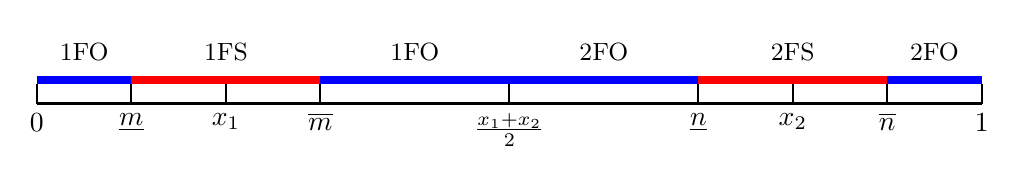
\begin{tikzpicture}[x=1.2cm]
\draw[black,thick,>=latex]
  (0,0) -- (10,0);%

\node[below,align=left,anchor=north,inner xsep=0pt]
  at (0,0) {$0$};	
\node[below,align=left,anchor=north,inner xsep=0pt]
  at (1,0) {$\underline{m}$};
\node[below,align=left,anchor=north,inner xsep=0pt]
  at (2,0) {$x_1$};
\node[below,align=left,anchor=north,inner xsep=0pt]
  at (3,0) {$\overline{m}$};
\node[below,align=left,anchor=north,inner xsep=0pt]
  at (5,0) {$\tfrac{x_1+x_2}{2}$};
\node[below,align=left,anchor=north,inner xsep=0pt]
  at (7,0) {$\underline{n}$};
\node[below,align=left,anchor=north,inner xsep=0pt]
  at (8,0) {$x_2$};
\node[below,align=left,anchor=north,inner xsep=0pt]
  at (9,0) {$\overline{n}$};
\node[below,align=left,anchor=north,inner xsep=0pt]
  at (10,0) {$1$};

\foreach \Xc in {0,1,2,3,5,7,8,9,10}
{
  \draw[black,thick]
    (\Xc,0) -- ++(0,7pt) node[above] {};
}

 \fill[red]
    (1,0.25)
      rectangle node[above, color=black] {\strut\small 1FS}
    (3,0.35);

 \fill[red]
    (7,0.25)
      rectangle node[above, color=black] {\strut\small 2FS}
    (9,0.35);

 \fill[blue]
    (0,0.25)
      rectangle node[above, color=black] {\strut\small 1FO}
    (1,0.35);

 \fill[blue]
    (3,0.25)
      rectangle node[above, color=black] {\strut\small 1FO}
    (5,0.35);

 \fill[blue]
    (5,0.25)
      rectangle node[above, color=black] {\strut\small 2FO}
    (7,0.35);

 \fill[blue]
    (9,0.25)
      rectangle node[above, color=black] {\strut\small 2FO}
    (10,0.35);

\end{tikzpicture}

\end{document}